\chapter{Теоретические сведения о системных вызовах fork и exec}

\section{Системный вызов fork}

\begin{figure}[ph!]
	\center{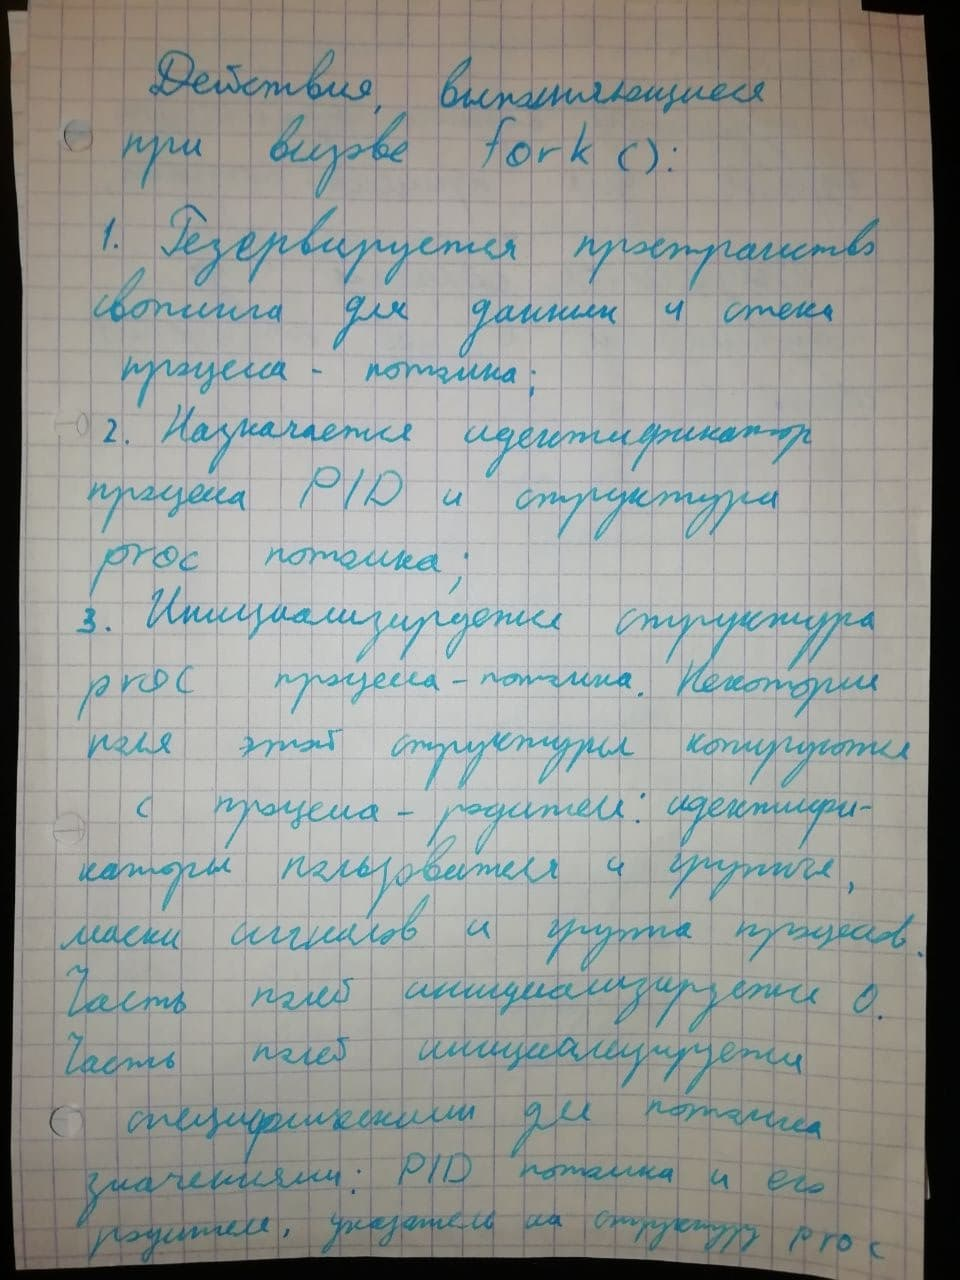
\includegraphics[scale=0.35]{fork_1}}
	\caption{Конспект fork - часть 1}
\end{figure}

\begin{figure}[ph!]
	\center{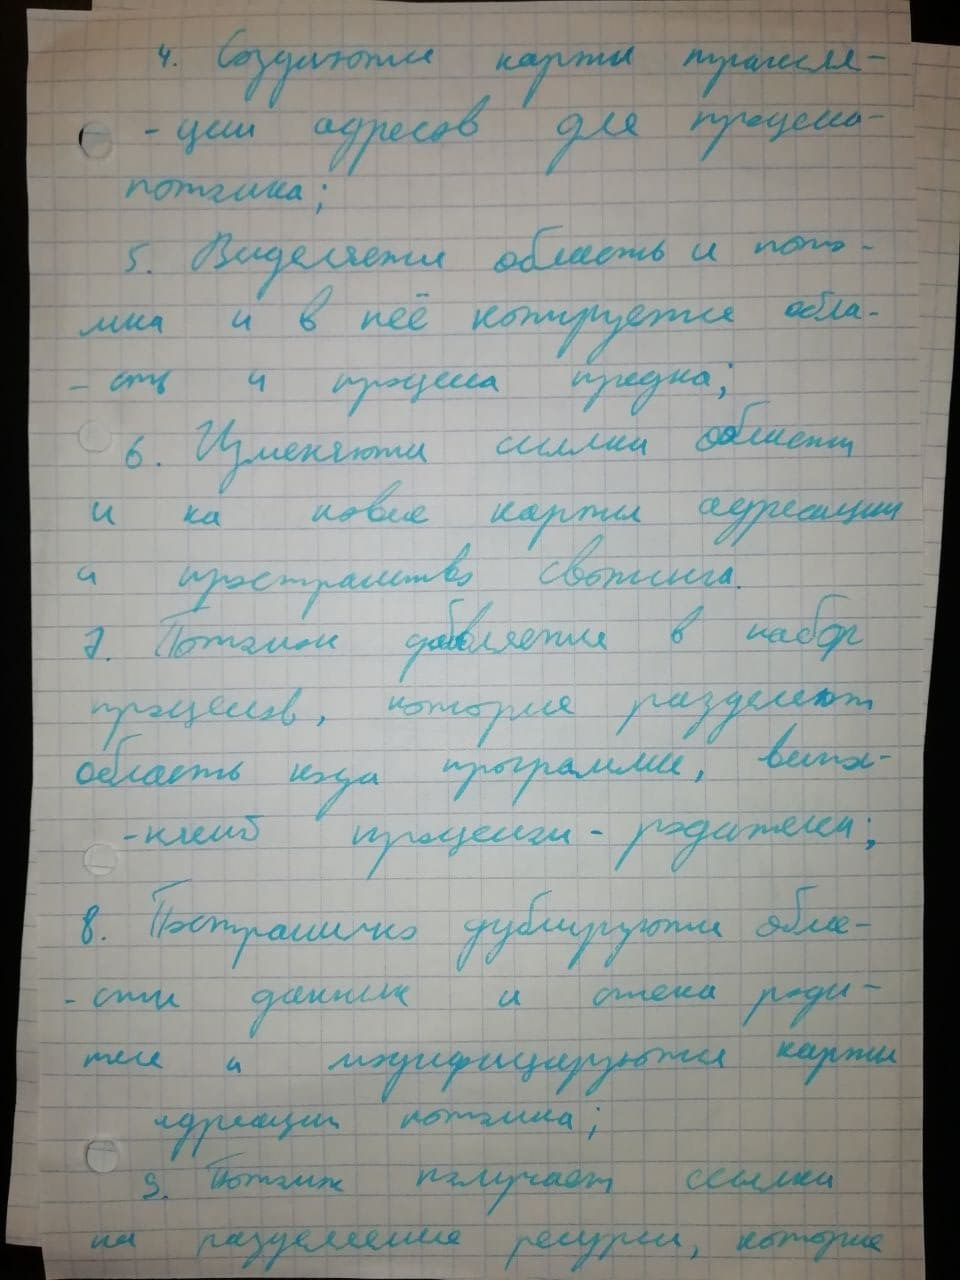
\includegraphics[scale=0.35]{fork_2}}
	\caption{Конспект fork - часть 2}
\end{figure}

\newpage

\begin{figure}[ph!]
	\center{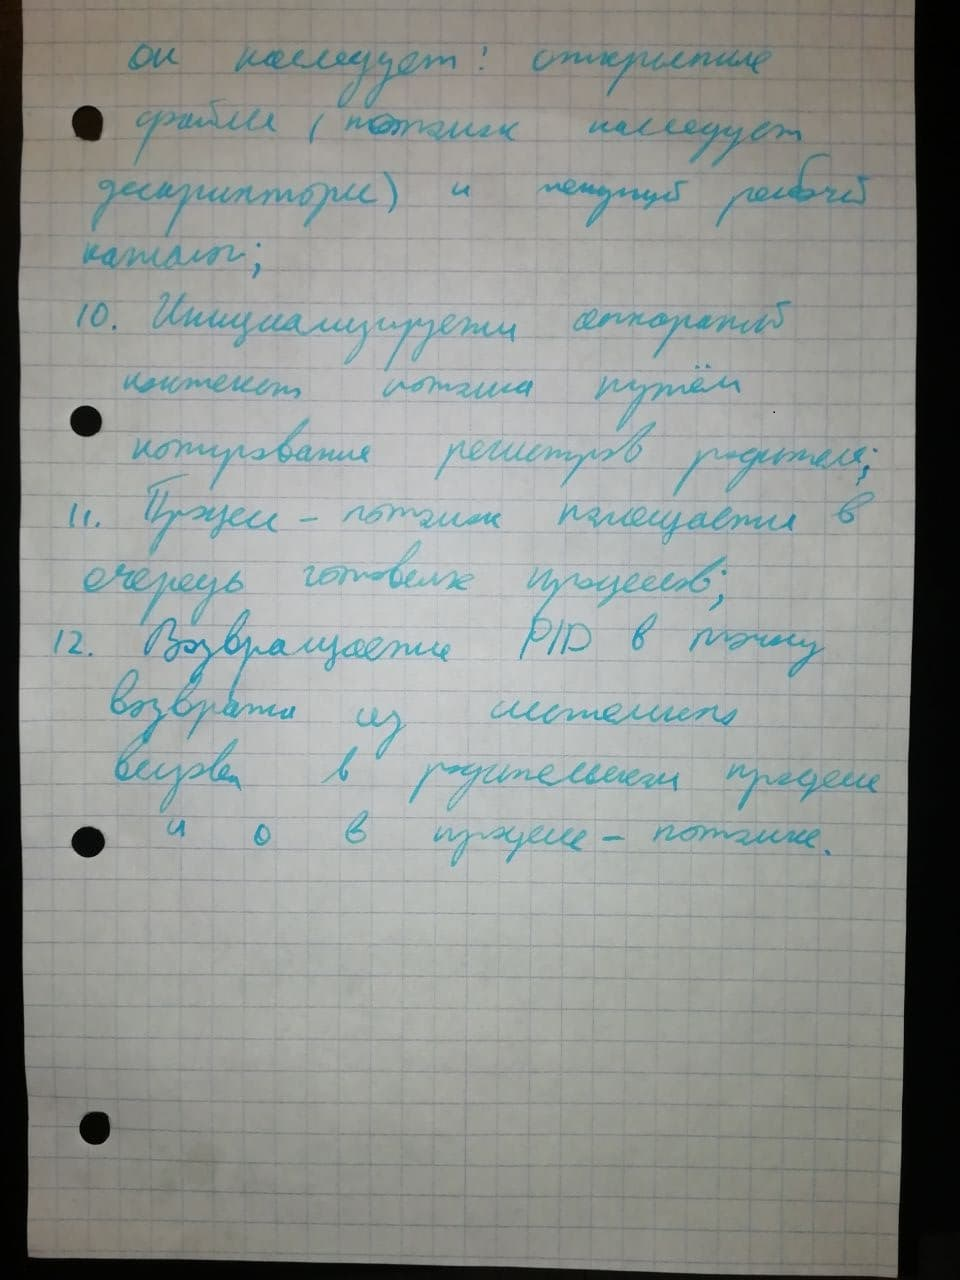
\includegraphics[scale=0.35]{fork_3}}
	\caption{Конспект fork - часть 3}
\end{figure}

\section{Системный вызов exec}

\begin{figure}[ph!]
	\center{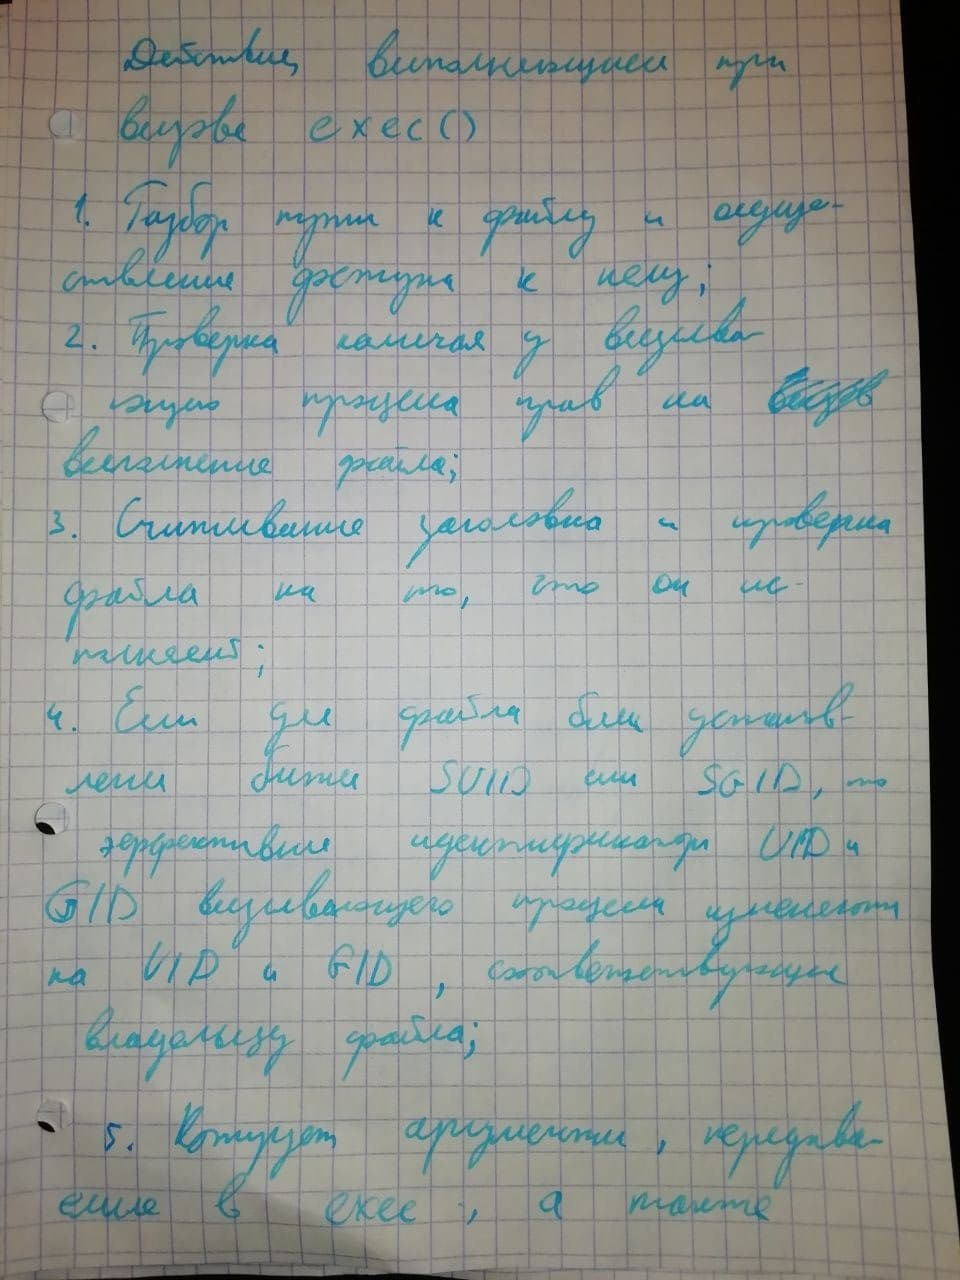
\includegraphics[scale=0.35]{exec_1}}
	\caption{Конспект exec - часть 1}
\end{figure}

\begin{figure}[ph!]
	\center{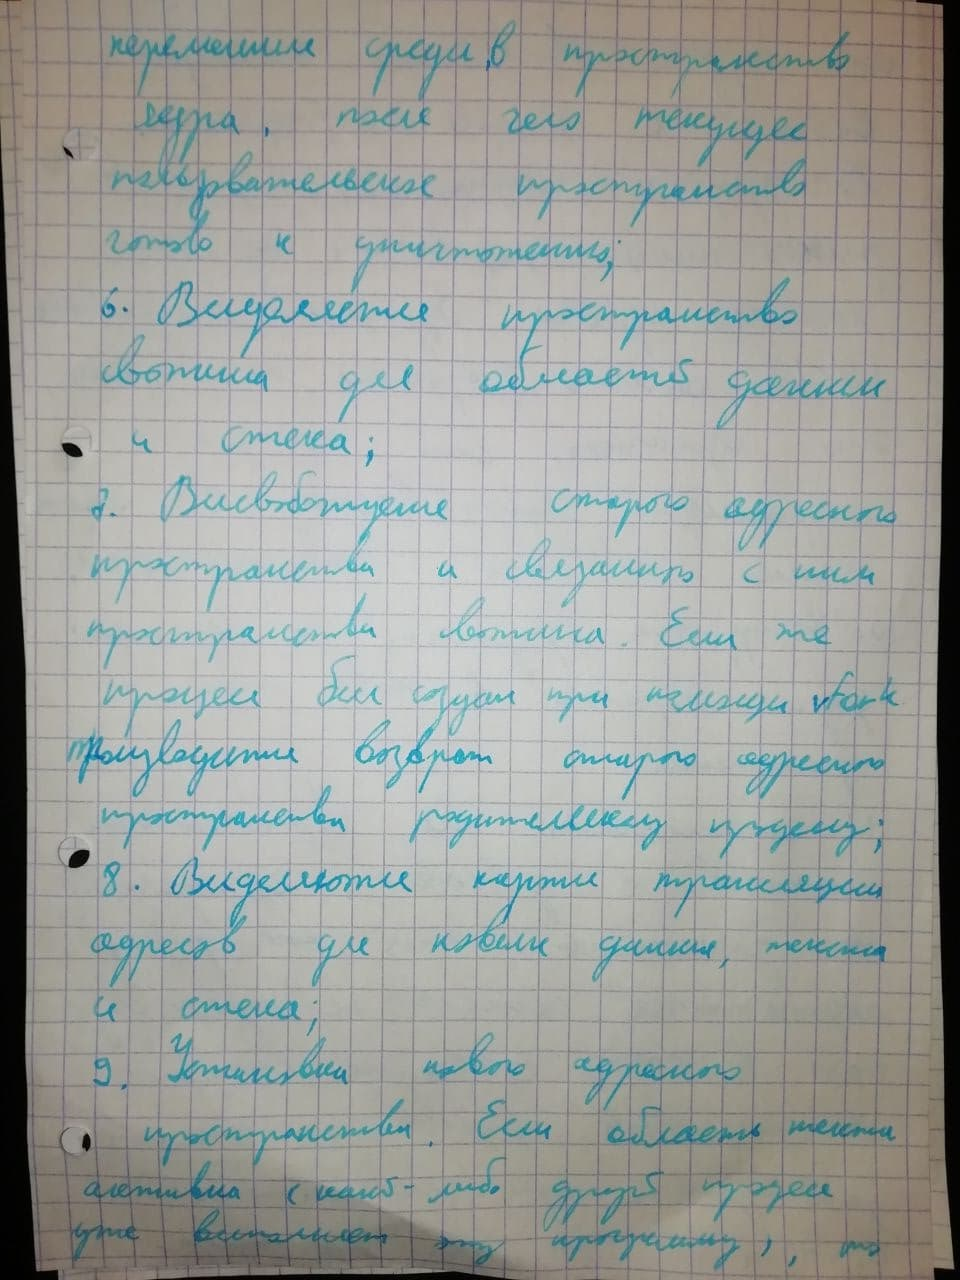
\includegraphics[scale=0.35]{exec_2}}
	\caption{Конспект exec - часть 2}
\end{figure}

\begin{figure}[ph!]
	\center{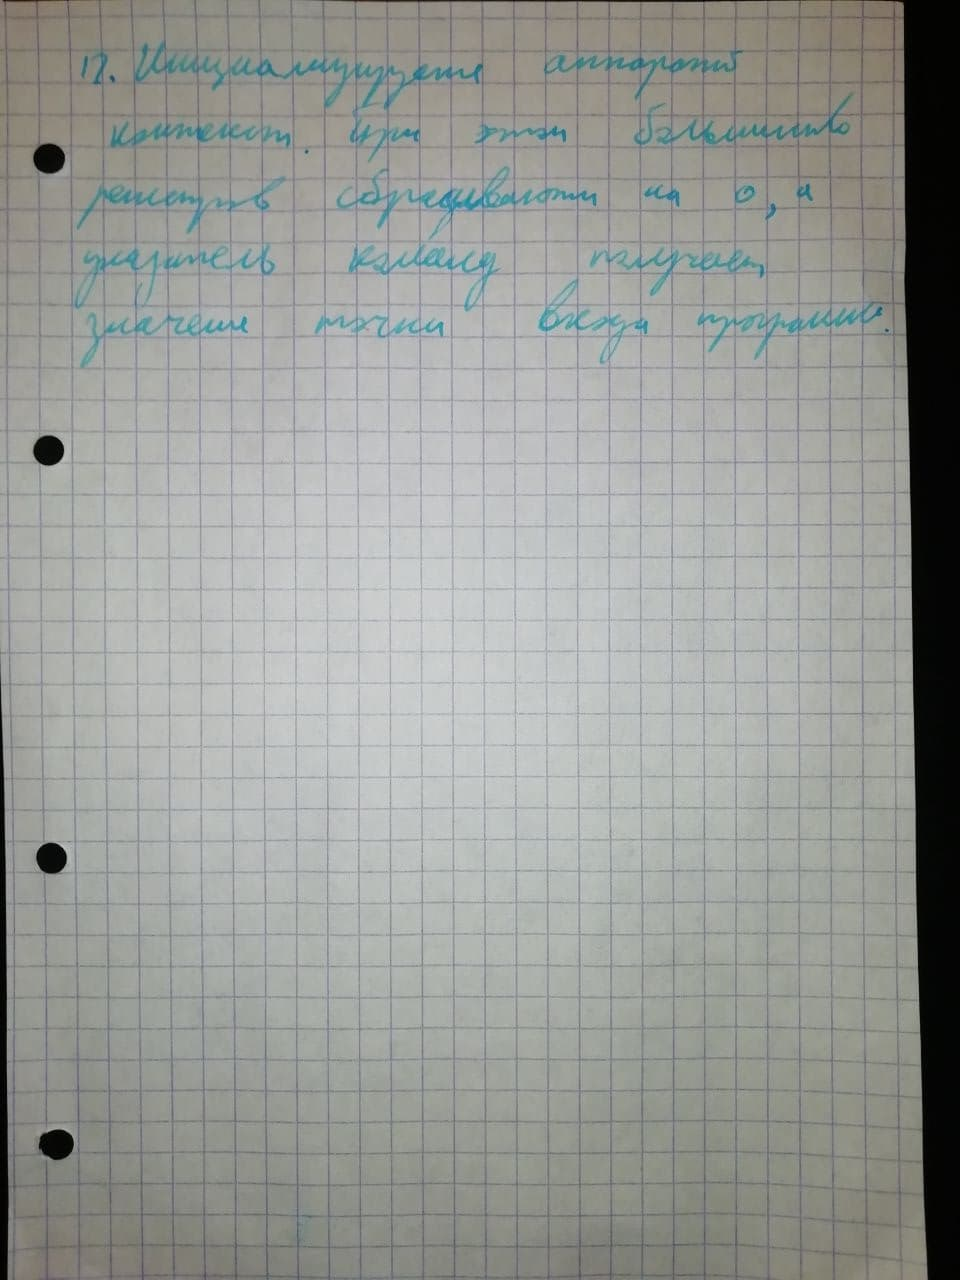
\includegraphics[scale=0.35]{exec_3}}
	\caption{Конспект exec - часть 3}
\end{figure}

\chapter{Листинг программ и результаты их работы}
\section{Задание №1}
Написать программу, запускающую не мене двух новых процессов системным вызовом fork(). В предке вывести собственный идентификатор (функция getpid()), идентификатор группы ( функция getpgrp())  и идентификаторы потомков. В процессе-потомке вывести собственный идентификатор, идентификатор предка (функция getppid()) и идентификатор группы. Убедиться, что при завершении процесса-предка потомок, который продолжает выполняться, получает идентификатор предка (PPID), равный 1 или идентификатор процесса-посредника.

\begin{lstlisting}[label=task_1,caption=Код к заданию №1]
#include <stdio.h>
#include <stdlib.h>
#include <unistd.h>

#define SLEEP_TIME 2

int pid;
int child_pid_1;
int child_pid_2;

int main(void)
{
    printf("Parent process|pid: \%d|group: \%d\\n", getpid(), getpgrp());

    child_pid_1 = fork();
    if (child_pid_1 == -1)
    {
        perror("Error: fork cannot be executed!");
        return 1;
    }
    else if (child_pid_1 == 0)
    {
        sleep(SLEEP_TIME);
        printf("Child 1 process|pid: \%d|ppid: \%d|group: \%d\\n", getpid(), getppid(), getpgrp());
        exit(0);
    }

    child_pid_2 = fork();
    if (child_pid_2 == -1)
    {
        perror("Error: fork cannot be executed!");
        return 1;
    }
    else if (child_pid_2 == 0)
    {
        sleep(SLEEP_TIME);
        printf("Child 2 process|pid: \%d|ppid: \%d|group: \%d\n", getpid(), getppid(), getpgrp());
        exit(0);
    }
    printf("Child PIDs of parent process|child 1: \%d|child 2: \%d\\n", child_pid_1, child_pid_1);
    printf("End of parent process\\n");
    return 0;
}
\end{lstlisting}

\begin{figure}[ph!]
	\center{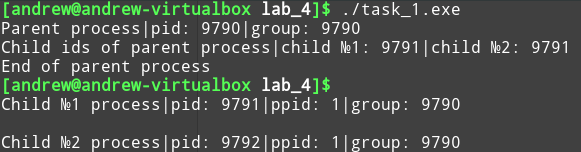
\includegraphics[scale=1.0]{task_1_result}}
	\caption{Результат работы программы}
\end{figure}

\section{Задание №2}
Написать программу по схеме первого задания, но в процессе-предке выполнить системный вызов wait(). Убедиться, что в этом случае идентификатор процесса потомка на 1 больше идентификатора процесса-предка.

\begin{lstlisting}[label=task_2,caption=Код к заданию №2]
#include <stdio.h>
#include <stdlib.h>
#include <unistd.h>

#include <sys/types.h>
#include <sys/wait.h>

#define SLEEP_TIME 2

int pid;
int child_pid_1;
int child_pid_2;

int main(void)
{
    printf("Parent process|pid: \%d|group: \%d\\n", getpid(), getpgrp());

    child_pid_1 = fork();
    if (child_pid_1 == -1)
    {
        perror("Error: fork cannot be executed!");
        return 1;
    }
    else if (child_pid_1 == 0)
    {
        printf("Child 1 process|pid: \%d|ppid: \%d|group: \%d\\n", getpid(), getppid(), getpgrp());
        exit(0);
    }

    child_pid_2 = fork();
    if (child_pid_2 == -1)
    {
        perror("Error: fork cannot be executed!");
        return 1;
    }
    else if (child_pid_2 == 0)
    {
        printf("Child 2 process|pid: \%d|ppid: \%d|group: \%d\\n", getpid(), getppid(), getpgrp());
        exit(0);
    }

    int return_status[2];
    pid_t child_pid[2];
    for (int i = 0; i < 2; i++)
    {
        child_pid[i] = wait(&(return_status[i]));
        printf("Child process finished|pid = \%d|status = \%d\\n", child_pid[i], return_status[i]);
        int status_value;
        if (WIFEXITED(status_value))
        {
            printf("Child process exited succesfully with code \%d\\n", WEXITSTATUS(status_value));
        }
        else
        {
            printf("Child process terminated abnormally\\n");
        }
    }
   
    printf("Child pids of parent process|child 1: \%d|child 2: \%d\\n", child_pid_1, child_pid_1);
    printf("End of parent process\\n");
    return 0;
}
\end{lstlisting}

\begin{figure}[ph!]
	\center{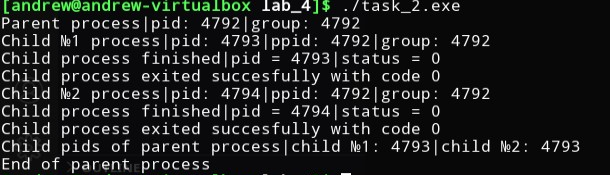
\includegraphics[scale=1.0]{task_2_result}}
	\caption{Результат работы программы}
\end{figure}

\section{Задание №3}
Написать программу, в которой процесс-потомок вызывает системный вызов exec(), а процесс-предок ждет завершения процесса-потомка. Следует создать не менее двух потомков.

\begin{lstlisting}[label=task_3,caption=Код к заданию №3]
#include <stdio.h>
#include <stdlib.h>
#include <sys/types.h>
#include <sys/wait.h>
#include <unistd.h>

int pid;
int child_pid_1;
int child_pid_2;

int main(void)
{
    printf("Parent process|pid: \%d|group: \%d\\n", getpid(), getpgrp());

    child_pid_1 = fork();
    if (child_pid_1 == -1)
    {
        perror("Error: fork cannot be executed!");
        return 1;
    }
    else if (child_pid_1 == 0)
    {
        printf("Child 1 process|pid: \%d|ppid: \%d|group: \%d\\n", getpid(), getppid(), getpgrp());
        int exec_result = execlp("/media/sf_manjaro_shared/BMSTU/OS/labs/lab_4/test/test_sort_str.exe", "gadfasf", 0);
        if (exec_result == -1)
            perror("Error: execlp cannot be executed!");
            return 2;
    }

    child_pid_2 = fork();
    if (child_pid_2 == -1)
    {
        perror("Error: fork cannot be executed!");
        return 1;
    }
    else if (child_pid_2 == 0)
    {
        printf("Child 2 process|pid: \%d|ppid: \%d|group: \%d\\n", getpid(), getppid(), getpgrp());
        int exec_result = execlp("/media/sf_manjaro_shared/BMSTU/OS/labs/lab_4/test/test_min_max.exe", "10", "5", "-1", "15", 0);
        if (exec_result == -1)
            perror("Error: execlp cannot be executed!");
            return 2;
    }

    int return_status[2];
    pid_t child_pid[2];
    for (int i = 0; i < 2; i++)
    {
        child_pid[i] = wait(&(return_status[i]));
        printf("Child process finished|pid = \%d|status = \%d\\n", child_pid[i], return_status[i]);
        int status_value;
        if (WIFEXITED(status_value))
        {
            printf("Child process exited succesfully with code \%d\\n", WEXITSTATUS(status_value));
        }
    }

    printf("Child pids of parent process|child 1: \%d|child 2: \%d\\n", child_pid_1, child_pid_1);
    printf("End of parent process\\n");
    return 0;
}
\end{lstlisting}

\newpage

\begin{figure}[ph!]
	\center{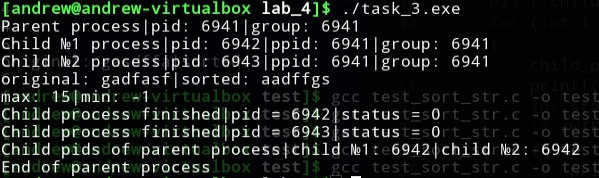
\includegraphics[scale=1.0]{task_3_result}}
	\caption{Результат работы программы}
\end{figure}

\section{Задание №4}
Написать программу, в которой предок и потомок обмениваются сообщением через программный канал.

\begin{lstlisting}[label=task_4,caption=Код к заданию №4]
#include <stdio.h>
#include <stdlib.h>
#include <sys/types.h>
#include <string.h>
#include <sys/wait.h>
#include <unistd.h>

int pid;
int child_pid_1;
int child_pid_2;

int main(void)
{
    printf("Parent process|pid: \%d|group: \%d\\n", getpid(), getpgrp());

    int message_pipe[2];
    if (pipe(message_pipe) == -1)
    {
        perror("Error: pipe cannot be executed!");
        return 1;
    }

    child_pid_1 = fork();
    if (child_pid_1 == -1)
    {
        perror("Error: fork cannot be executed!");
        return 1;
    }
    else if (child_pid_1 == 0)
    {
        printf("Child 1 process|pid: \%d|ppid: \%d|group: \%d\\n", getpid(), getppid(), getpgrp());
        close(message_pipe[0]);
        write(message_pipe[1], "message from child 1", strlen("message from child 1") + 1);
        printf("Message was sent to parent from child 1\\n");
        return 0;
    }

    child_pid_2 = fork();
    if (child_pid_2 == -1)
    {
        perror("Error: fork cannot be executed!");
        return 1;
    }
    else if (child_pid_2 == 0)
    {
        printf("Child 2 process|pid: \%d|ppid: \%d|group: \%d\\n", getpid(), getppid(), getpgrp());
        close(message_pipe[0]);
        write(message_pipe[1], "message from child 2", strlen("message from child 2") + 1);
        printf("Message was sent to parent from child 2\\n");
        return 0;
    }

    int return_status[2];
    pid_t child_pid[2];
    for (int i = 0; i < 2; i++)
    {
        child_pid[i] = wait(&(return_status[i]));
        printf("Child process finished|pid = \%d|status = \%d\\n", child_pid[i], return_status[i]);
        int status_value;
        if (WIFEXITED(status_value))
        {
            printf("Child process exited succesfully with code \%d\\n", WEXITSTATUS(status_value));
        }
    }

    char buff_1[24] = {0};
    char buff_2[24] = {0};
    close(message_pipe[1]);
    read(message_pipe[0], buff_1, sizeof(buff_1));
    read(message_pipe[0], buff_2, sizeof(buff_2));
    printf("Received message from child: \%s\\n", buff_1);
    printf("Received message from child: \%s\\n", buff_2);
    printf("Child pids of parent process|child 1: \%d|child 2: \%d\\n", child_pid_1, child_pid_1);
    printf("End of parent process\\n");
    return 0;
}
\end{lstlisting}

\begin{figure}[ph!]
	\center{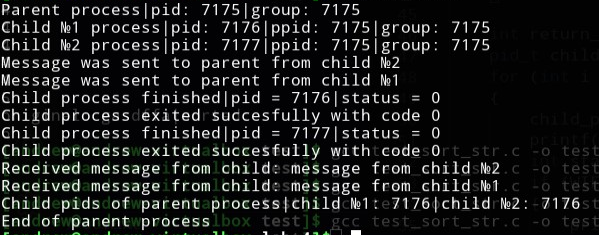
\includegraphics[scale=1.0]{task_4_result}}
	\caption{Результат работы программы}
\end{figure}

\section{Задание №5}
В программу с программным каналом включить собственный обработчик сигнала. Использовать сигнал для изменения хода выполнения программы.

\begin{lstlisting}[label=task_5,caption=Код к заданию №5]
#include <signal.h>
#include <stdio.h>
#include <stdlib.h>
#include <string.h>
#include <sys/types.h>
#include <sys/wait.h>
#include <unistd.h>

int pid;
int child_pid_1;
int child_pid_2;

int signal_state = 0;

void ignore_signal(int signal) {printf("test");}
void writing(int signal) {printf("test"); signal_state = 1;}

int main(void)
{
    printf("Parent process|pid: \%d|group: \%d\\n", getpid(), getpgrp());

    int message_pipe[2];
    if (pipe(message_pipe) == -1)
    {
        perror("Error: pipe cannot be executed!");
        return 1;
    }

    signal(SIGINT, ignore_signal);
    child_pid_1 = fork();
    if (child_pid_1 == -1)
    {
        perror("Error: fork cannot be executed!");
        return 1;
    }
    else if (child_pid_1 == 0)
    {
        signal(SIGINT, writing);
        sleep(5);
        if (signal_state == 1)
        {
            printf("Child 1 process|pid: \%d|ppid: \%d|group: \%d\\n", getpid(), getppid(), getpgrp());
            close(message_pipe[0]);
            write(message_pipe[1], "message from child 1", strlen("message from child 1") + 1);
            printf("Message was sent to parent from child 1\\n");
        }
        else
        {
            printf("No signal was sent\\\n");
        }
        return 0;
    }

    child_pid_2 = fork();
    if (child_pid_2 == -1)
    {
        perror("Error: fork cannot be executed!");
        return 1;
    }
    else if (child_pid_2 == 0)
    {
        signal(SIGINT, writing);
        sleep(5);
        if (signal_state == 1)
        {
            printf("Child 2 process|pid: \%d|ppid: \%d|group: \%d\\n", getpid(), getppid(), getpgrp());
            close(message_pipe[0]);
            write(message_pipe[1], "message from child 2", strlen("message from child 2") + 1);
            printf("Message was sent to parent from child 2\\n");
        }
        else
        {
            printf("No signal was sent\\n");
        }
        return 0;
    }

    int return_status[2];
    pid_t child_pid[2];
    for (int i = 0; i < 2; i++)
    {
        child_pid[i] = wait(&(return_status[i]));
        printf("Child process finished|pid = \%d|status = \%d\\n", child_pid[i], return_status[i]);
        int status_value;
        if (WIFEXITED(status_value))
        {
            printf("Child process exited succesfully with code \%d\\n", WEXITSTATUS(status_value));
        }
    }

    char buff_1[24] = {0};
    char buff_2[24] = {0};
    close(message_pipe[1]);
    read(message_pipe[0], buff_1, sizeof(buff_1));
    read(message_pipe[0], buff_2, sizeof(buff_2));
    printf("Received message from child: \%s\\n", buff_1);
    printf("Received message from child: \%s\\n", buff_2);
    printf("Child pids of parent process|child 1: \%d|child 2: \%d\\n", child_pid_1, child_pid_1);
    printf("End of parent process\\n");
    return 0;
}
\end{lstlisting}

\begin{figure}[ph!]
	\center{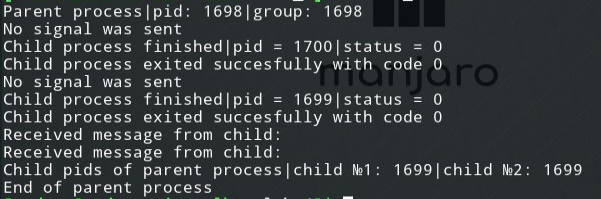
\includegraphics[scale=1.0]{task_5_result_no_signal}}
	\caption{Результат работы программы без сигнала}
\end{figure}

\begin{figure}[ph!]
	\center{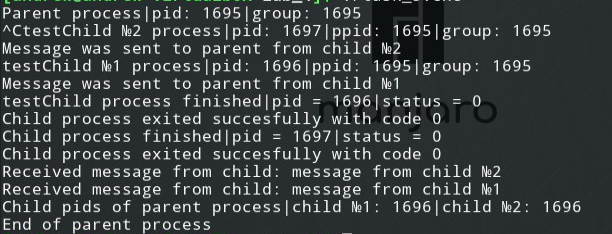
\includegraphics[scale=1.0]{task_5_result_signal}}
	\caption{Результат работы программы с сигналом}
\end{figure}
